\colorbox{white!10!}{
    \begin{minipage}{0.2\textwidth}
       \begin{flushleft}
        \includegraphics[width = 0.6\textwidth]{Эмблема.png}
       \end{flushleft}
    \end{minipage}
    \begin{minipage}[t]{0.7 \textwidth}
        \begin{center}
            {\huge \textsc{Красноярская Летняя Школа. Сезон $7^2 - 2$}}
            \vspace{0.25cm}
            
            { \huge \textbf{ФМТ. Тур 5.2}}
        \end{center}
        \vspace{0.05cm}
    \end{minipage}
}

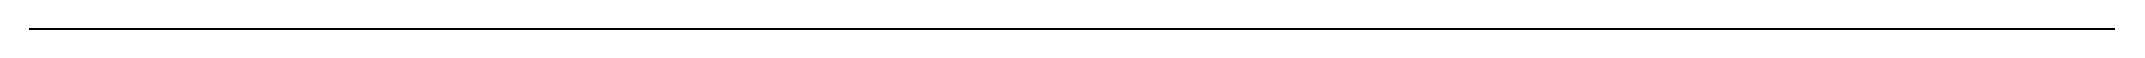
\begin{tikzpicture}
    \draw[thick] (-6.5,0)--(20,0);
\end{tikzpicture}
\begin{enumerate}
    \item Два мальчика тянут веревку в разные стороны, прикладывая к ней силы $F$ каждый. Веревка выдерживает подвешенные к ней грузы массой до 15 кг. При каких значениях $F$ верёвка не порвётся?

    \item Атлет бежит по круглому стадиону радиуса $r$, с постоянной по модулю скоростью $v$. Найти среднюю скорость перемещения спортсмена в момент времени $t = \tau$.
    
\end{enumerate}